\documentclass[11pt]{IEEEtran}

% ========================= Packages =========================
\usepackage{graphicx}
\usepackage{float}
\usepackage{pgfplots}
\usepackage{pgfplotstable}
\usepackage{csvsimple}
\usepackage{tikz}
\usepackage{circuitikz}
\usepackage{siunitx}
\usepackage{booktabs}
\usepackage{hyperref}
\usepackage{multirow}
\usepackage{tabularx}
\usepackage{nicematrix}
\usepackage{array}

%\usepackage{cite}

\pgfplotsset{compat=newest}

% ========================= Project Commands =========================
\newcommand{\comet}{C.O.M.E.T.}
\newcommand{\ares}{A.R.E.S.}
\newcommand{\phobos}{P.H.O.B.O.S.}
\newcommand{\deimos}{D.E.I.M.O.S.}
\newcommand{\insight}{INSIGHT}
\newcommand{\RHeight}{12}

\begin{document}


%=================================================================================
%Outlines Report Guidelines

%%%%%%%% Needs Project Title, Names of Team Members, Instructors, and Advisors %%%%%%%%%%%%%%%%%

\onecolumn

\newcommand{\Space}{\\[.5cm]}
%\lhead{A.U.R.O.R.A.}
%\chead {}
%\rhead{\comet}
\begin{center}
    \vfill
    \textbf{\Large AURORA Rocket and Experimental Systems (A.R.E.S.)}
\vfill
  \begin{figure}[h]
    \centering
    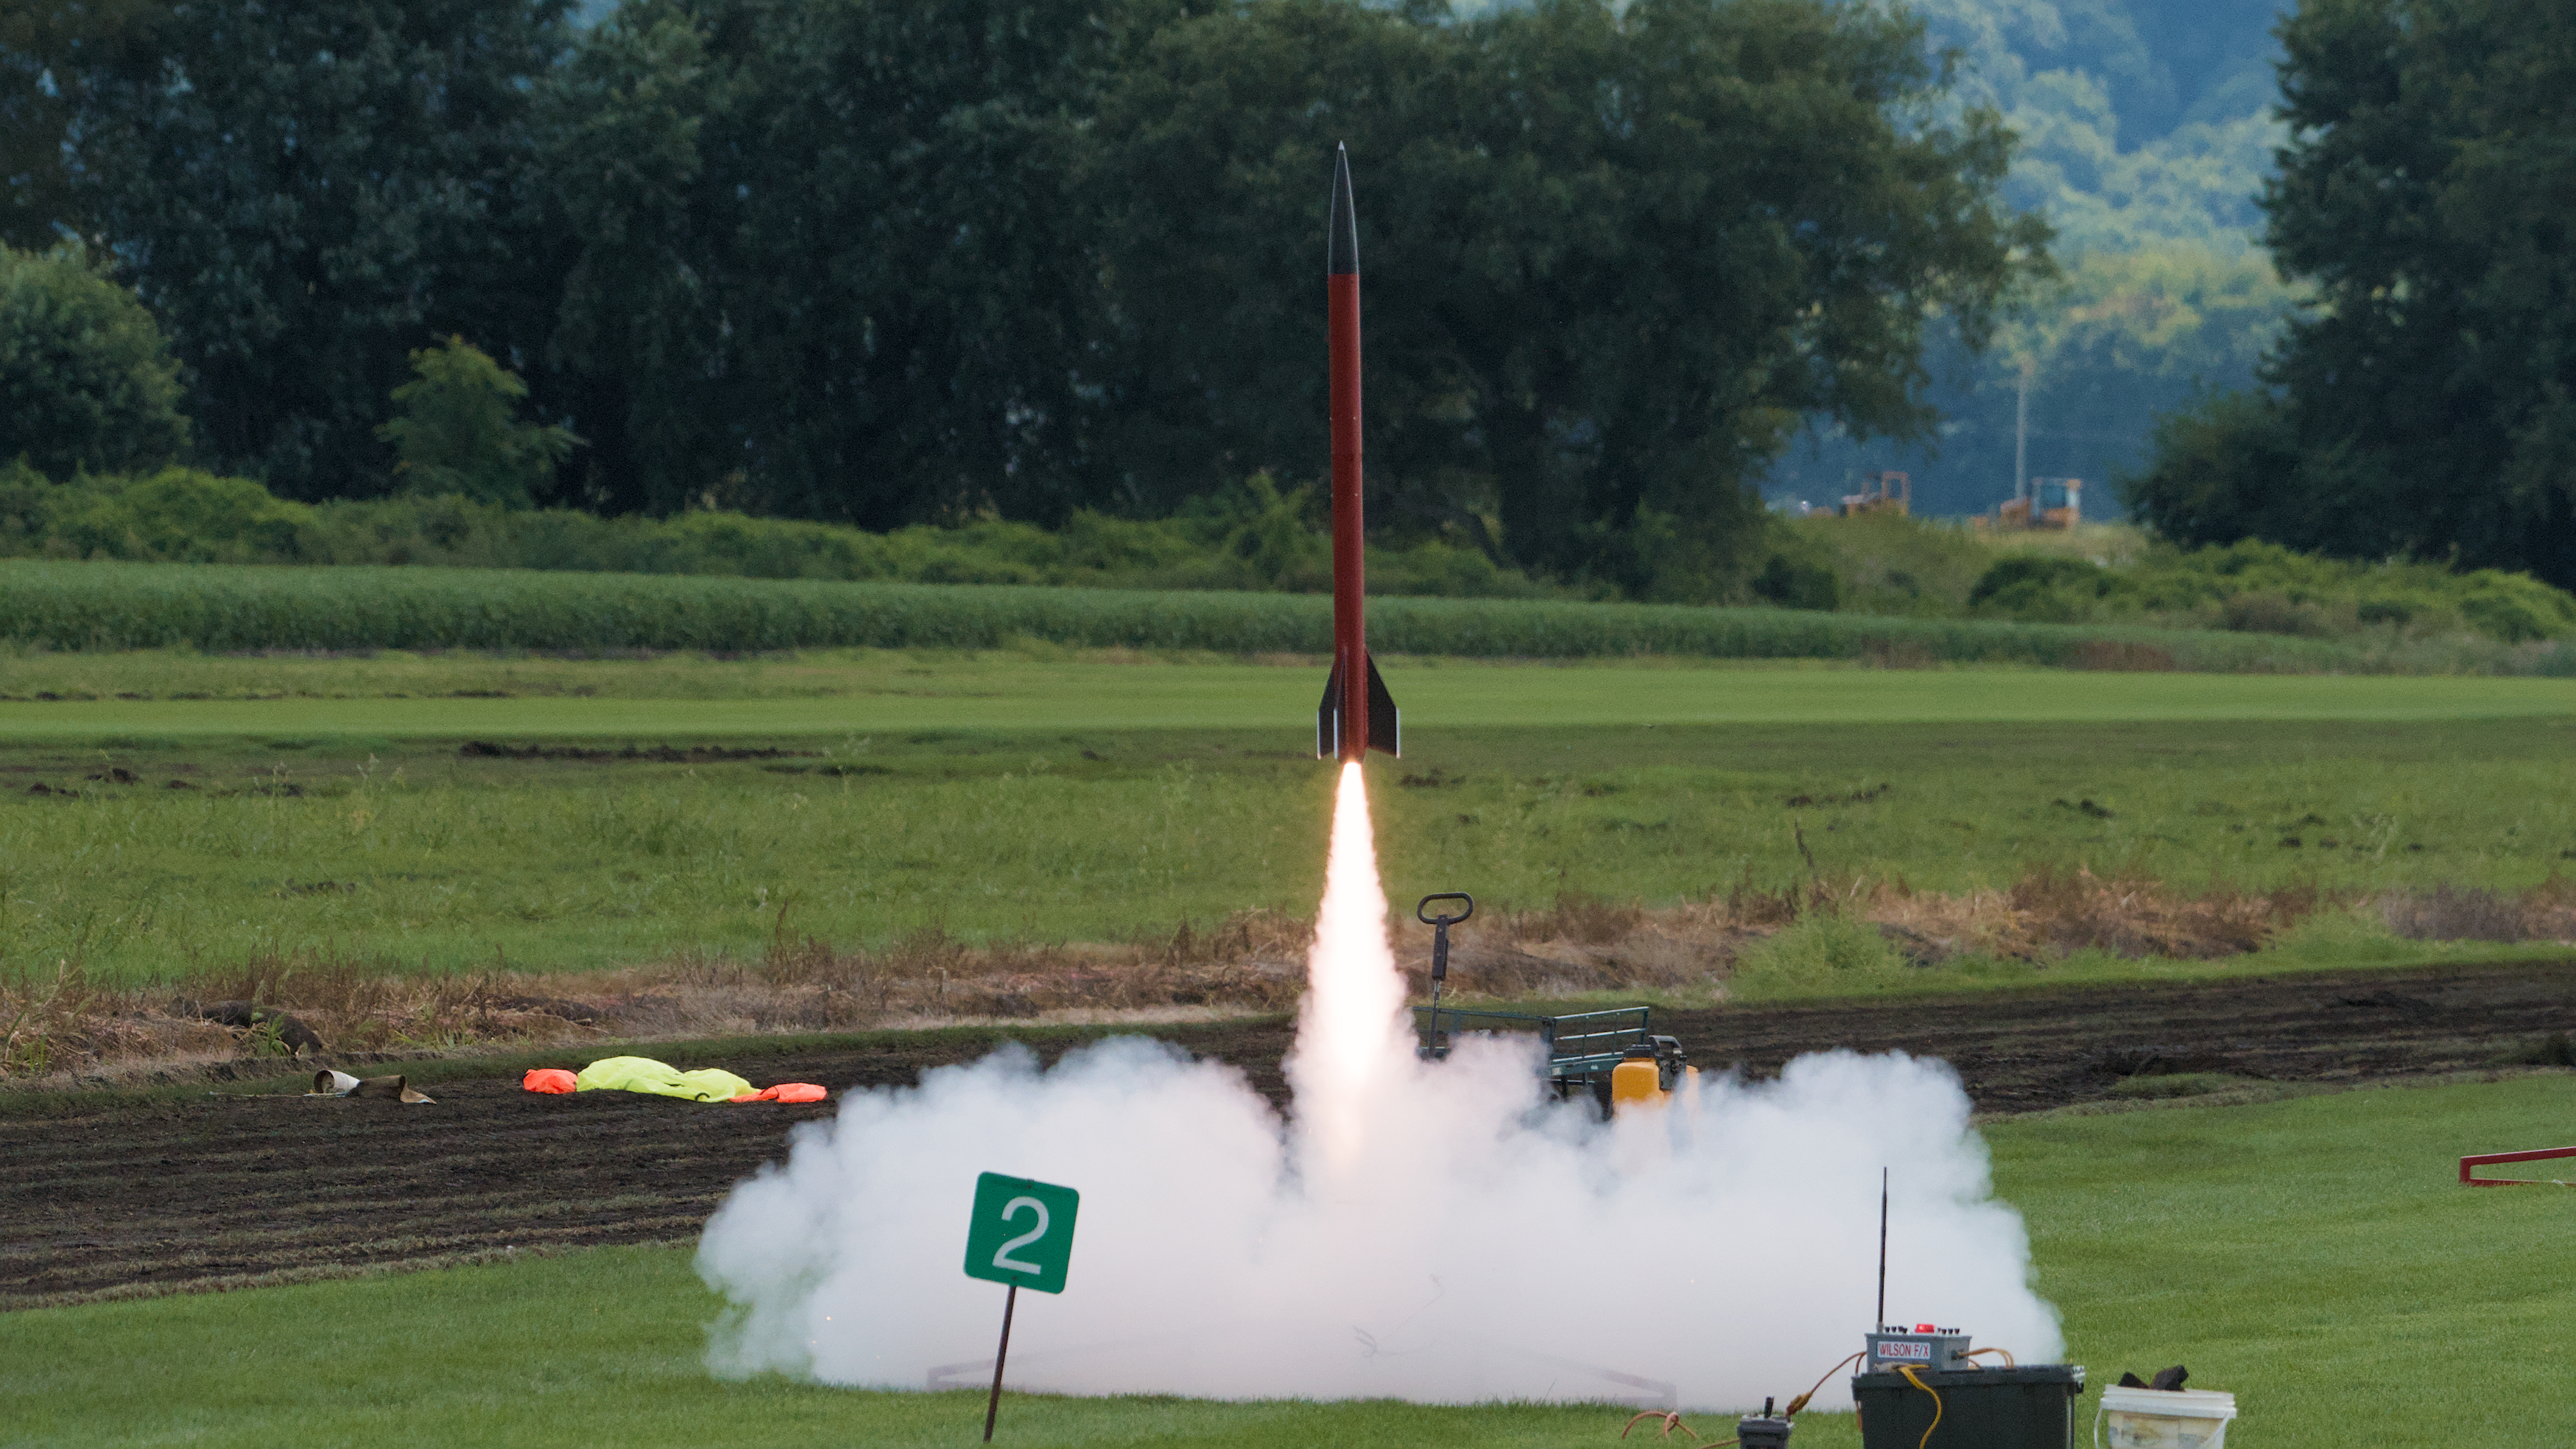
\includegraphics[trim={2cm 0 0 0}, clip,width=1\linewidth]{Documentation//ARES/Cover_Photo.jpg}
    \label{fig:placeholder}
\end{figure}
        

    \vfill
    \author[Kyle Eckert,
    \author[Nicholas Krupa,
    \author[Liam Gordon
    \vfill

    Technical Advisors\\Dr. Patricia Mellodge, Professor Allan Penda, Professor Loel Goldblatt \vfill
    Instructors\\Dr. Ying Yu, Dr. Xin Shen, Professor Jean Goulart\vfill
    \today

    \newpage
    
\end{center}

\onecolumn
\tableofcontents
\newpage
%Need report writing Contribution Tables

\onecolumn
%\section{Project Team and Roles}

\begin{IEEEbiography}
[{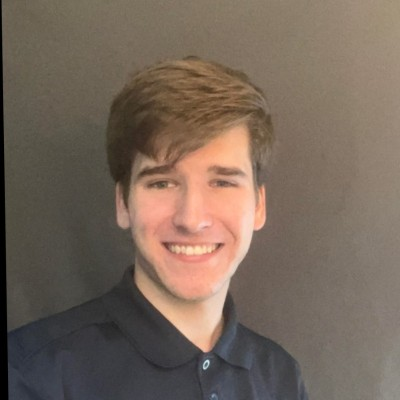
\includegraphics[width=1in,height=1.25in,clip,keepaspectratio]{Headshots/NHeadshot.jpg}}]
{\normalsize Nicholas Krupa}
\normalsize
is a senior electrical engineering major with minors in physics and mathematics. He is the founder and president of the AURORA Rocketry Team, a Senior Research Assistant within the Multiscale Metamaterial Research Laboratory, and holds a Level 2 High Power Rocketry certification through the National Association of Rocketry. He is a recipient of both a NASA Connecticut Space Grant Consortium Undergraduate Scholarship and an Undergraduate Research Grant for his work on phased-array antennas for satellite and space communication \cite{ctsgcSpring2024,ctsgcFall2024}. He is also a co-author of published research involving microwave metasurface design and characterization \cite{wells2024}. For this project, he will coordinate the overall \ares{} mission, including vehicle requirements, subsystem integration, flight operations, and development of the \deimos{} telemetry system and \comet{} flight computer. His previous experience includes leading the University of Hartford NASA RockSat-C team and developing several generations of custom high-power rocketry avionics. He completed an engineering internship with Ensign-Bickford Aerospace \& Defense (EBAD) during Summer 2026 and has accepted a full-time return offer with the company following graduation.
\end{IEEEbiography}

\begin{IEEEbiography}
[{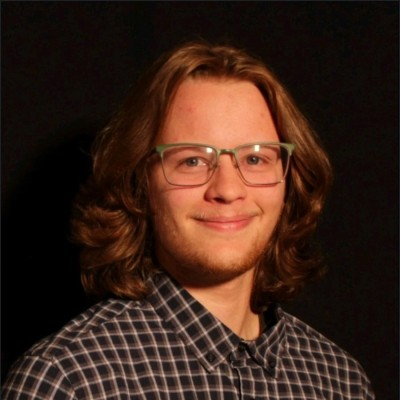
\includegraphics[width=1in,height=1.25in,clip,keepaspectratio]{Headshots/KHeadshot.jpg}}]
{\normalsize Kyle Eckert}

\normalsize
is a senior electrical engineering major with minors in audio engineering and mathematics and serves as the electrical lead for the Multiscale Metamaterial Research Laboratory. His work in the laboratory focuses on the design and development of experimental instrumentation for characterizing material properties at microwave frequencies. He also designs modifications to existing measurement systems to expand their operational and measurement capabilities. He was awarded a NASA Connecticut Space Grant Consortium Undergraduate Research Grant during the Spring 2026 award cycle for research involving rocket-based RF and metamaterial communication systems \cite{ctsgc2026}. Kyle was also the Lead Electrical Engineer and Flight Engineer with the 2026 RockSat program, where he designed and developed circuitry to enable experiments to fly aboard NASA sounding rockets and collect data under flight conditions. He holds a Level 1 High Power Rocketry certification and is a co-creator of the \comet{} dual-deployment system, a four-layer PCB-based avionics system. He will lead the design, fabrication, and testing of the \phobos{} phased-array antenna payload, with emphasis on RF electronics, antenna systems, and communication engineering.
\end{IEEEbiography}



\begin{IEEEbiography}
[{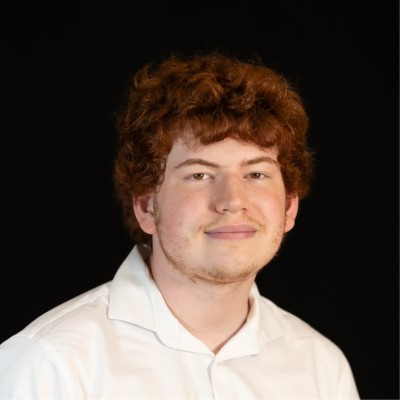
\includegraphics[width=1in,height=1.25in,clip,keepaspectratio]{Headshots/LHeadshot.jpg}}]
{\normalsize Liam Gordon}
\normalsize
is a senior mechanical engineering major, president of the University of Hartford AIAA Student Chapter, and vice president of the AURORA Rocketry Team. He holds a Level 1 High Power Rocketry certification and has contributed to multiple student aerospace design and flight projects. His work on AURORA was recognized as one of the Top 3 Sophomore Projects at the University of Hartford's Spring 2025 CETA Design Expo \cite{uhartexpo2025}. He also participated in the University's inaugural AIAA Design/Build/Fly team, competing in Tucson, Arizona in 2025 \cite{uhartdbf2025}. Through the competition, he gained hands-on experience in aircraft design, CAD, fabrication, technical inspection, field testing, and rapid mechanical troubleshooting. He has additionally contributed to NASA Connecticut Space Grant-supported high-power rocketry work through AURORA. For the \ares{} project, he will lead vehicle mechanical design and manufacturing, including aerodynamic and structural analysis, CAD development, material selection, computational fluid dynamics, and finite element analysis. He will also oversee fabrication, mechanical integration, and structural verification of the completed vehicle.

\end{IEEEbiography}
\newpage



%\section{Introduction}

\section{Use Case}
%Detailed Use Case (10 Points)

%This section focuses on demonstrating the practical application of your capstone project through  a detailed and realistic use case. Address the following points in two subsections.  2.1 Use Case Overview Provide a clear and detailed description of the use case for the product that your capstone  design project will deliver. Explain the role your project plays in designing and developing this  product. If you have more technical use-case illustrations or diagrams, include them here to support your explanation. 2.2. Practical Scenario Present a realistic scenario that demonstrates how the product will be used by the intended user(s). Address the following: i. Purpose: Clearly state why the product is being designed and the specific problem or need it addresses. ii. User/Customer Description: Define the target audience for your product. Who will  benefit from it, and what are their key characteristics or requirements? iii. Usage Context: Describe the context in which the product will be used. Include details about: • Where: The environment or setting (e.g., home, workplace, public spaces). • When: The timing or conditions under which the product is most likely to be used. • How: The manner in which the product is expected to function or be interacted with by the user.Make sure your description is clear, engaging, and supported by relevant examples or visuals to help illustrate the use case"

\subsection{Overview}
The AURORA Rocket and Experimental Systems (\ares{}) project is a student-developed, modular high-power sounding rocket being designed by the University of Hartford's AURORA rocketry team.
Its immediate use case is participation in the 2027 International Rocket Engineering Competition (IREC), in the 10,000-foot commercial-off-the-shelf (COTS) propulsion category.
The vehicle is intended to carry an experimental communications payload while providing the structural, avionics, and recovery functions needed to perform and document a safe research flight.
The proposed vehicle is approximately \RHeight{}~ft long, 6~in in diameter, and constructed primarily from fiberglass.
The mission target is 10,000~ft above ground level (AGL), not a demonstrated flight result.
IREC eligibility, launch procedures, and payload integration will be checked against the applicable 2027 competition documents \cite{irecRules,irecGuide}.

Three student-developed electronic subsystems address different mission needs.
\phobos{} is a scientific phased-array payload that evaluates directional communication and electronic beam steering from a translating and rotating rocket.
\deimos{} is a nose-cone flight-instrumentation and telemetry module that measures position, pressure-derived altitude, acceleration, and vehicle attitude.
\comet{} is a flight-event and dual parachute deployment controller that detects ascent and descent events, records measurements, and commands the drogue and main recovery parachute outputs.
The broader \ares{} structure, propulsion section, harnesses, parachutes, and ground equipment connect these subsystems into a single mission.

Beyond its competition objectives, A.R.E.S. serves as an educational and research platform developed in collaboration with the University of Hartford's Multiscale Metamaterial Research Laboratory.
This collaboration integrates the laboratory's ongoing research in microwave and metamaterial technologies into the P.H.O.B.O.S. phased-array antenna payload, extending laboratory-based research into a dynamic, real-world flight environment.
By evaluating the performance of an electronically steered antenna aboard a sounding rocket, the project aims to advance research into directional communication systems for future aerospace applications.
Consequently, mission success is defined not only by achieving the competition altitude target, but also by collecting meaningful RF and flight-performance data and safely recovering the vehicle and experimental hardware for postflight analysis and continued research.

\subsection{Practical Scenario}
%Devlopment of practical skills outside of the classroom in a high pace structured environment like a rocketry competition?
The primary users of \ares{} are student engineers within the University of Hartford's AURORA Rocketry Club and faculty researchers seeking a reusable platform for testing experimental avionics, communication systems, and aerospace technologies.
The project is developed in collaboration with the University's Multiscale Metamaterial Research Laboratory, with the goal of extending laboratory research in microwave and antenna technologies into a realistic flight environment.

Development of the project is supported by Ensign-Bickford Aerospace \& Defense (EBAD), which provides funding for the rocket's development, and the NASA Connecticut Space Grant Consortium, which funds development of the \phobos{} phased-array antenna payload.
Together, these efforts provide an opportunity to demonstrate experimental communication technologies while developing the infrastructure and experience necessary for future student aerospace research.

A representative application of \ares{} is its participation in the 2027 International Rocket Engineering Competition (IREC) in Midland, Texas.
The competition provides a structured environment in which the team must design, construct, test, and launch a sounding rocket targeting an altitude of approximately 10,000~ft AGL while carrying an experimental payload.
This mission allows the team to evaluate whether the developed systems can operate reliably under the acceleration, vibration, rotation, and environmental conditions experienced during flight.

Prior to launch, the team integrates the vehicle's electronic subsystems, verifies electrical connections and battery operation, and inspects the structural and recovery hardware.
The RF team evaluates antenna performance and communication with the ground station, while the mechanical team verifies the vehicle's structural interfaces, motor retention, and recovery equipment.
The recovery systems are checked and armed according to the applicable range safety procedures \cite{tripoliCode}.

During flight, \deimos{} measures and records the rocket's position, acceleration, and orientation while transmitting telemetry to the ground station.
Simultaneously, \phobos{} investigates electronically steered communication using a 2.4-GHz phased-array antenna.
By adjusting the relative phase of its antenna elements in response to the rocket's orientation, the payload will attempt to maintain a directional communication link with the receiving ground station.
The resulting measurements will allow researchers to evaluate phased-array performance under dynamic flight conditions rather than exclusively within a laboratory.

The \comet{} flight computer monitors onboard sensors to identify flight events and initiate the dual-parachute recovery sequence.
The drogue parachute is commanded at apogee, followed by the main parachute at a proposed altitude of approximately 700~ft AGL.
A separate commercial deployment altimeter is also planned to provide an independent recovery system.

Following landing, the team recovers the rocket and downloads the recorded flight data.
Measurements from \deimos{} and \phobos{} are compared to investigate the relationship between vehicle orientation, antenna steering, and received signal performance.
Flight data is also compared against simulations to evaluate vehicle performance and identify potential design improvements.

Success is therefore measured not only by achieving the competition altitude target and safely recovering the vehicle, but also by obtaining meaningful experimental data that supports continued research within the Multiscale Metamaterial Research Laboratory and future development of the AURORA program.
% We are making a rocket as part of the UHart rocketry club AURORA, to compete in ERSA IREC. the goal of this is to advance the clubs and therefore the scfhools aerospace research as well as to further the research done by the multiscale metamaterial research lab by implimenting the research into its stated application of space communication. this is done by putting a phased array antenna inside the rocket as a payload. this also serves the purpose of meeting IRECs experimental payload challenge.

\section{Requirements and Specifications}
% What do the systems need to be qualified as functional. 


\subsection{Engineering Standards and Codes}
% Needs to compley to local laws and reguklations such as FCC transmission NPFA 1127 and part 101 that govern high power rocketry, as well as the competion rules for ERSA IREC. 

\subsection{Ethical Considerations}
%Making a rocket that uses pytechnics 
\subsection{Requirements and Specifications Table}
% For the nose cone tracking system (Insight) it needs to fit within the rocket nose cone tranmit at a far enough range to be recied at max rocket height of 10K Feet work off battery power, Needs to have a GPS reciever and full size right angle sma port for rgitity (NO UFL or wire wip). It also needs to be able to track the rockets full orentation in flight complete with abasoulte postion tracking roll pitch yaw accelration in three axis and gravity vecotr output and baromter. Must meet all FCC and Comepttion requirements inclsuign max tramission power SRAD frency allocations and no frequncy hoping.

% for example, phobos needs to operate at a frequency that balances cost of components, transmission range, and patch antenna size so it fits within rocket. it needs to fit within rocket frame, operate off of an onboard battery to work with linear regulators. it must meet all IREC requirements such as wire gauge. It must be able to transmit to the ground station from near apogee (10k ft). must adhere to FCC legal standards including power transmission. It must limit the number of deadzones that wont transmit to GND station. Must Connect securely to the rocket and to associated boards. 
\subsubsection*{\ares{} Rocket}
~\\


\subsubsection*{\deimos{} Nosecone Telemetry}
~\\

\subsubsection*{\phobos{} Scientific Payload}
~\\
\begin{table}[H]
    \centering
    \begin{tabular}{ccccp{6cm}}
    \toprule
       \textbf{Category}                    & \textbf{Metric}   & \textbf{Value Estimate}   & \textbf{Unit}  & \textbf{Notes}\\ \hline
       %
\multirow{3}{*}{\textbf{Physical}}   & Height            & $\leq 22$                 & in   & Must be contained within Rocket payload Canister \\ \cmidrule{2-5}
                                            & Diameter          & $\leq$ 6           &in    & System must be contained within rocket body tube\\ \cmidrule{2-5}
                                            & Mass              & $\leq$ 2           & kg   & Must meet IREC payload requirements and be controlled for rocket stability\\ \midrule
        \multirow{3}{*}{\textbf{Functional}}& Power Supply      & $~ 9$              & V    & Source must accomodate all systems in addition to lasting extended launch pad time \\ \cmidrule{2-5}
                                            & operating band    & 2.4                & \unit{\giga\hertz}     & Must operate in legal band, easy to impliment, and allow for good steering\\ \cmidrule{2-5}
                                            & Patch Layout      & 2x1x4              &   ---       & Must allow for efficient and controllable steering\\ \cmidrule{2-5}
                                            & Wire Guage        & $\leq22$           &   AWG       & Must be easy to use and meet IREC requirement \\ \cmidrule{2-5}
                                            & Connection        & Positively Retained& ---         & Must survive launch and landing forces \\ \cmidrule{2-5}
                                            & RF Interface      & SMA                & ---         & Must have low loss, fit within housing, and maintain secure connection\\ \midrule
        \multirow{3}{*}{\textbf{Performance}}&   Link Distance  & ~2                 &\unit{\kilo\meter} & Must retain connection for majority of flight \\ \cmidrule{2-5}                       
                                            & Steering coverage & $\pm 30$           & \unit{\deg} & Must have a measurable amount of active steering \\ \cmidrule{2-5}
                                            & Radiated Power    & $\leq 1$           &\unit{\watt} & Must meet the FCC legal transmission limit for amateur endeavors.\\ \bottomrule
    
    \end{tabular}
    \vspace{3mm}
    \caption{\phobos{} Scientific Payload}
    \label{tab:PhobosReq}
\end{table}

\subsubsection*{\comet{} Dual Parachute Deployment}
~\\

%COMET criteria
% Must have a samll footprint of 2.5"x1". Must be user-programable through a gui and USB-C. Must be able to store data onboard for flight analysis. Must utilize batteries that meet linear regulator requirements. must utilize sensors such as barometric altimeters and accelerometers to detect launch and apogee events and control triggering pyrotechnics. Must be externally arm-able for safety. must have audible alerts and continutiy checks. must be able to handle high currents for breif amounts of time. 

\section{Design}
% This section needs . KEY PRINCIPLES AND TECHNOLOGY INVESTIGATIONS.
%Kyle is focused on the FREQ that the PHOBOS System will be using and why that frequncy was chosen,

% Kyles frequency reasoning: A compromise had to be made between transmission range, price of components, and ease of implimentation. 915 required a patch size and spacing far too large for the rockets body to fit, 5Ghz had too low of a legal transmission range and increased the price of components significantly, although the patch spacing was much lower. 2.4Ghz provided a middle ground of the two. allowing for about 4 patches in height and a reasonable transmission range.

% Nick is wokring on what microcontroller shoul dbe used for these systems. MCU slection was based around ease of use and documentation avaible as well as multiple buses and wide range of GPIO to conform to the many proejcts we are undertaking. But has a flight hsitory for high power rocketry. without costing an arm and a leg. The Rp2040 emerged as a systemw e felt comfomtable using for each of our sunssytems as we have made dev baord with them before and prorgamming is very easy. 



\subsection{Key Principles, Strategy and Feasibility}
% after each FBD, discuss some of the key points and why decisions were made see phobos section for example


%\subsubsection{\ares{}}
%~\\
%\begin{figure}[H]
%    \centering
%    \includegraphics[width=.75\linewidth]{Documentation/Pics/ares_Block_Diagram.png}
%    \caption{}
%    \label{fig:ares_Block}
%\end{figure}


\subsubsection*{\deimos{}}
%This is the nose cone tracking system
~\\
\begin{figure}[H]
    \centering
    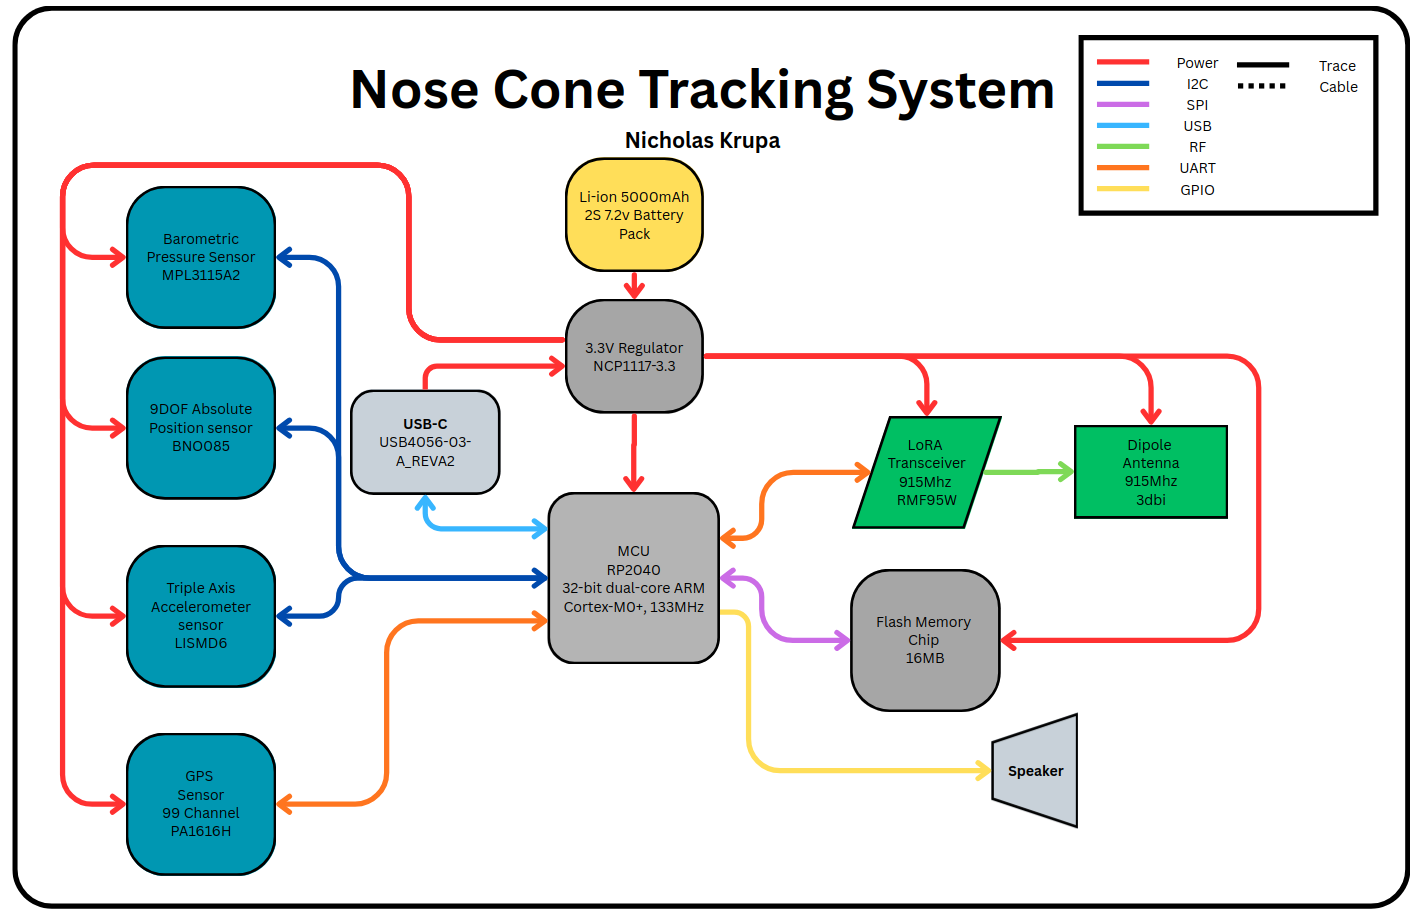
\includegraphics[width=.75\linewidth]{Documentation/Pics/NC_Block_Diagram.png}
    \caption{\deimos{} Nose cone telemetry functional block diagram}
    \label{fig:NC_Block}
\end{figure}


\subsubsection*{\phobos{}}
~\\
\begin{figure}[H]
    \centering
    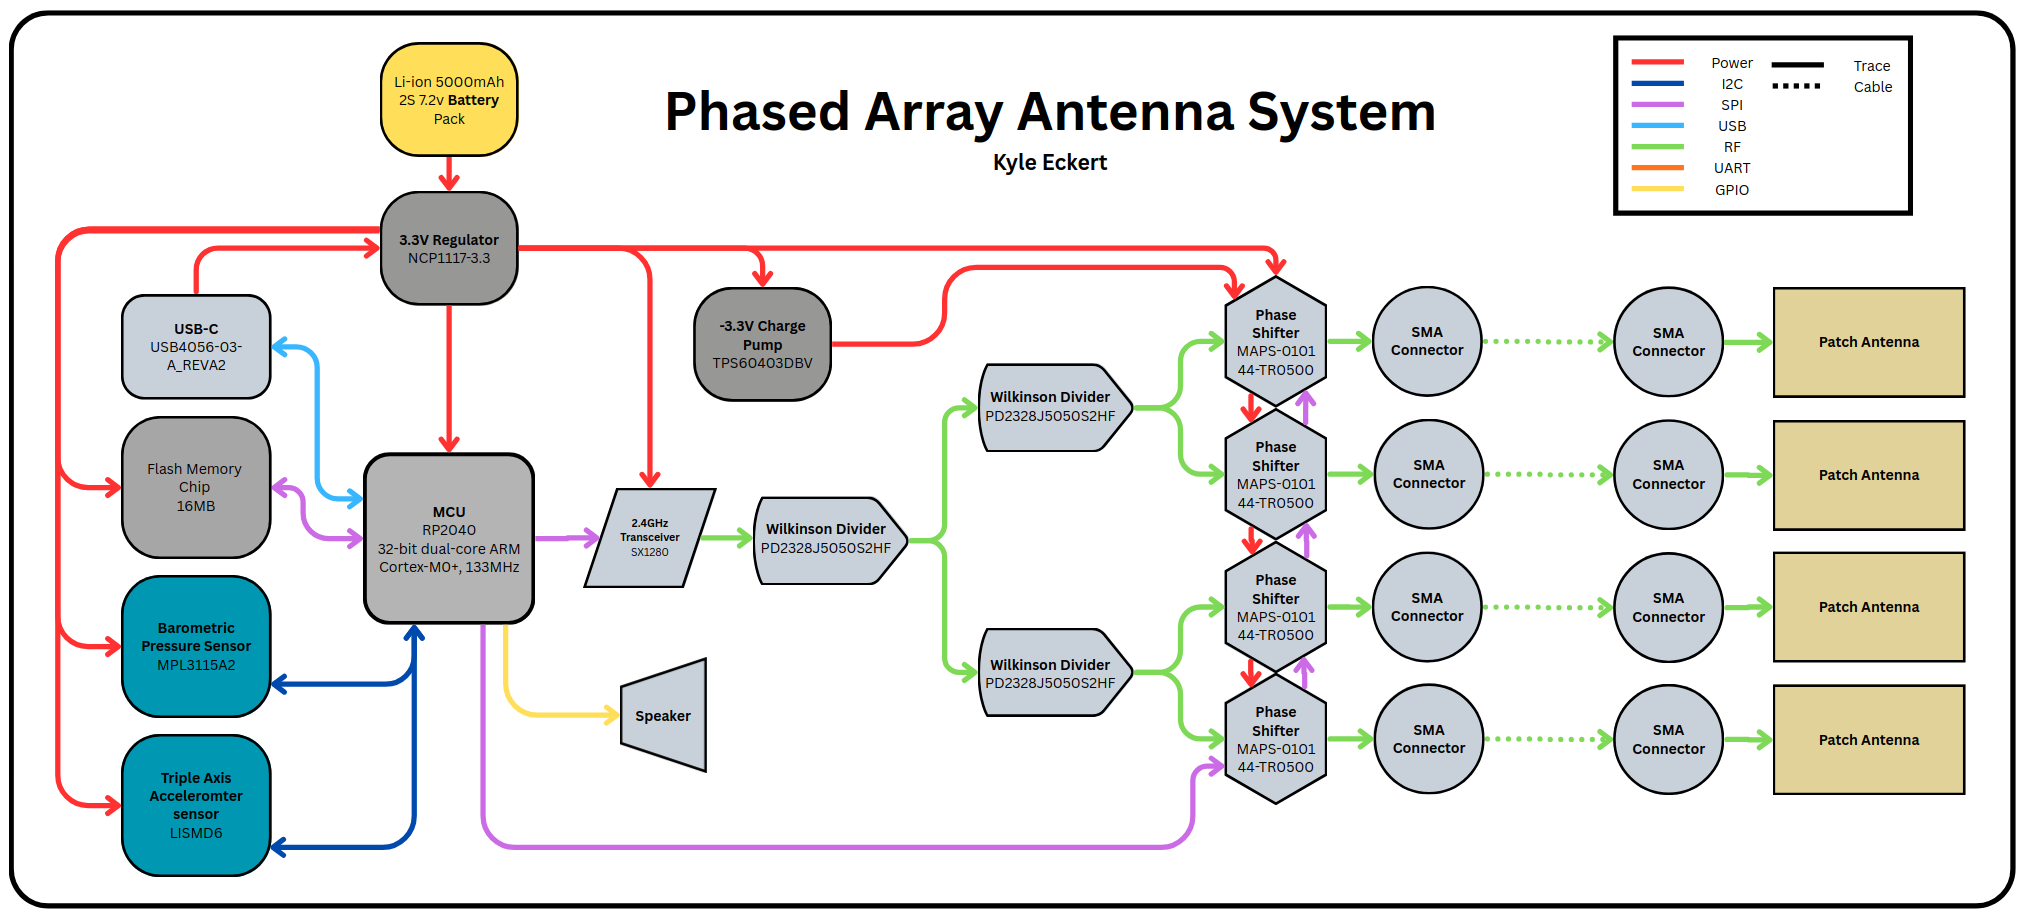
\includegraphics[width=.75\linewidth]{Documentation/Pics/PAA_Block_Diagram.png}
    \caption{}
    \label{fig:PHOBOS_Block}
\end{figure}
In a phased array, changing the phase of the signal at each antenna element steers the direction of constructive interference. Frequency affects the size and spacing of the patches, free-space path loss, and the available RF components. The team compared 915 MHz, 2.4 GHz, and 5 GHz as candidates. The 2.4-GHz band was chosen as the best packaging and implementation compromise for a six-inch rocket % add citation

A phased array requires a method of dividing the transmitted signal and controlling the phase at each patch. Digital phase shifters are preferred for repeatable MCU-controlled settings. Packaged power dividers and coaxial feeds reduce the amount of custom microwave layout required for an initial flight prototype, although their losses and phase errors still need measurement

\subsubsection*{\comet{}}
~\\
\begin{figure}[H]
    \centering
    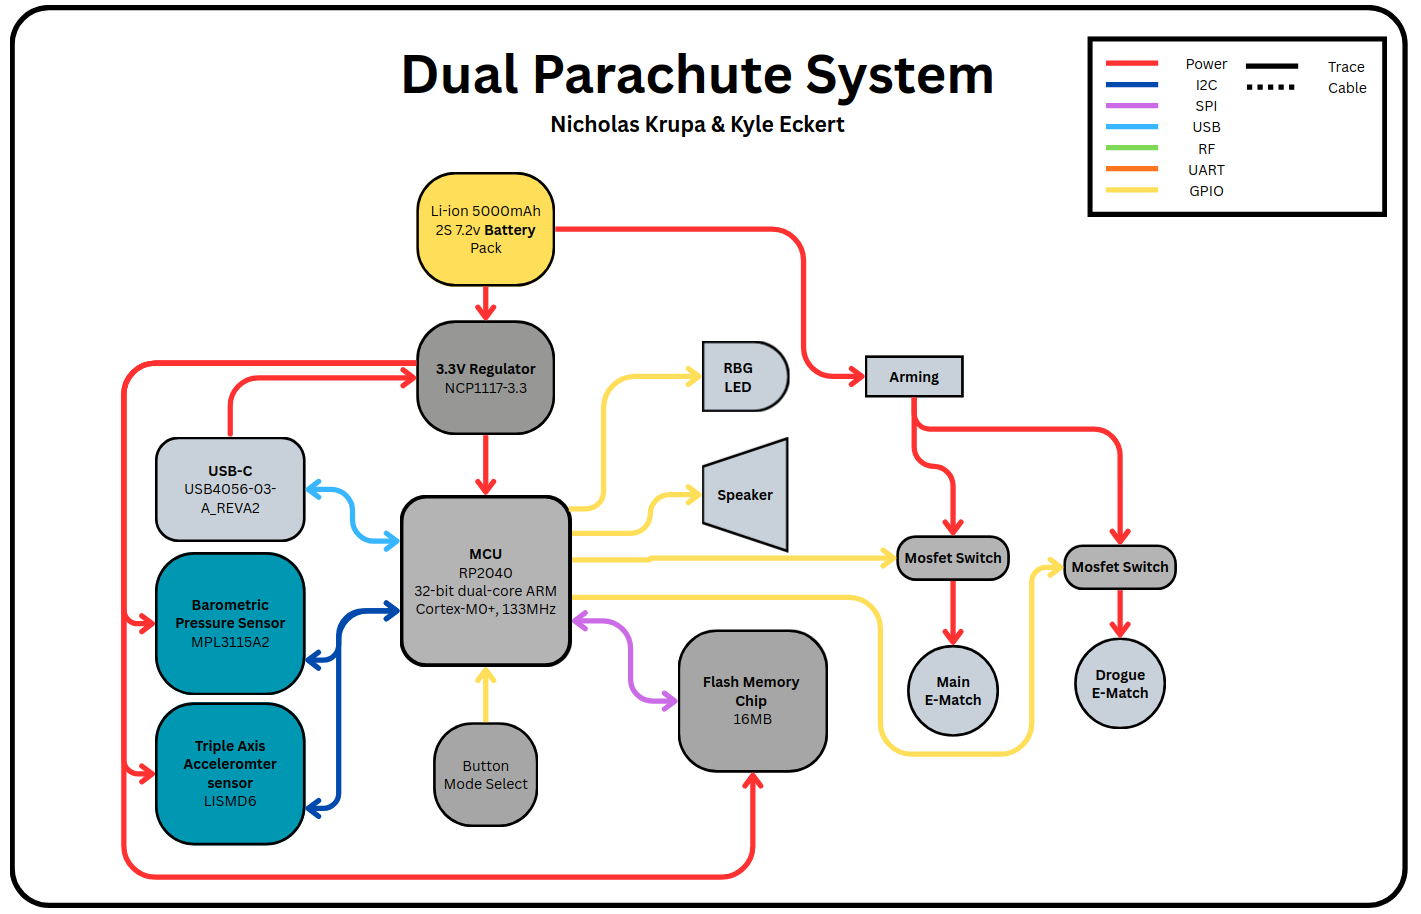
\includegraphics[width=.75\linewidth]{Documentation/Pics/DPS_Block_Diagram.png}
    \caption{}
    \label{fig:COMET_Block}
\end{figure}

\subsection{Investigations}

%\subsection{Ethical Consideration and Impacts on Design}

%\subsection{Design Elements}

%\subsection{Overall Design}


%\section{Projected Timeline}

%\subsection{Schedule Overview}

%\subsection{Numbered List of Tasks}

%\subsection{PERT Chart}

%\subsection{Gantt Chart}

%\subsection{Task Responsibility}


%\section{Budget}


\bibliographystyle{ieeetr}
\bibliography{Documentation/ARES/References}

\end{document}
